% Options for packages loaded elsewhere
\PassOptionsToPackage{unicode}{hyperref}
\PassOptionsToPackage{hyphens}{url}
\PassOptionsToPackage{dvipsnames,svgnames*,x11names*}{xcolor}
%
\documentclass[
]{article}
\usepackage{amsmath,amssymb}
\usepackage{lmodern}
\usepackage{ifxetex,ifluatex}
\ifnum 0\ifxetex 1\fi\ifluatex 1\fi=0 % if pdftex
  \usepackage[T1]{fontenc}
  \usepackage[utf8]{inputenc}
  \usepackage{textcomp} % provide euro and other symbols
\else % if luatex or xetex
  \usepackage{unicode-math}
  \defaultfontfeatures{Scale=MatchLowercase}
  \defaultfontfeatures[\rmfamily]{Ligatures=TeX,Scale=1}
\fi
% Use upquote if available, for straight quotes in verbatim environments
\IfFileExists{upquote.sty}{\usepackage{upquote}}{}
\IfFileExists{microtype.sty}{% use microtype if available
  \usepackage[]{microtype}
  \UseMicrotypeSet[protrusion]{basicmath} % disable protrusion for tt fonts
}{}
\makeatletter
\@ifundefined{KOMAClassName}{% if non-KOMA class
  \IfFileExists{parskip.sty}{%
    \usepackage{parskip}
  }{% else
    \setlength{\parindent}{0pt}
    \setlength{\parskip}{6pt plus 2pt minus 1pt}}
}{% if KOMA class
  \KOMAoptions{parskip=half}}
\makeatother
\usepackage{xcolor}
\IfFileExists{xurl.sty}{\usepackage{xurl}}{} % add URL line breaks if available
\IfFileExists{bookmark.sty}{\usepackage{bookmark}}{\usepackage{hyperref}}
\hypersetup{
  colorlinks=true,
  linkcolor=Maroon,
  filecolor=Maroon,
  citecolor=Blue,
  urlcolor=blue,
  pdfcreator={LaTeX via pandoc}}
\urlstyle{same} % disable monospaced font for URLs
\usepackage[margin=1in]{geometry}
\usepackage{graphicx}
\makeatletter
\def\maxwidth{\ifdim\Gin@nat@width>\linewidth\linewidth\else\Gin@nat@width\fi}
\def\maxheight{\ifdim\Gin@nat@height>\textheight\textheight\else\Gin@nat@height\fi}
\makeatother
% Scale images if necessary, so that they will not overflow the page
% margins by default, and it is still possible to overwrite the defaults
% using explicit options in \includegraphics[width, height, ...]{}
\setkeys{Gin}{width=\maxwidth,height=\maxheight,keepaspectratio}
% Set default figure placement to htbp
\makeatletter
\def\fps@figure{htbp}
\makeatother
\setlength{\emergencystretch}{3em} % prevent overfull lines
\providecommand{\tightlist}{%
  \setlength{\itemsep}{0pt}\setlength{\parskip}{0pt}}
\setcounter{secnumdepth}{-\maxdimen} % remove section numbering
\ifluatex
  \usepackage{selnolig}  % disable illegal ligatures
\fi

\author{}
\date{\vspace{-2.5em}}

\begin{document}

\hypertarget{diamonds}{%
\section{Diamonds}\label{diamonds}}

\hypertarget{examining-the-relationship-between-characteristics-of-a-diamond-and-its-price}{%
\subsection{Examining the relationship between characteristics of a
diamond and its
price}\label{examining-the-relationship-between-characteristics-of-a-diamond-and-its-price}}

\hypertarget{benson-chou}{%
\subsubsection{Benson Chou}\label{benson-chou}}

\hypertarget{march-10-2023}{%
\subsubsection{March 10, 2023}\label{march-10-2023}}

\hypertarget{introduction}{%
\subsection{Introduction}\label{introduction}}

Growing up, it is common to hear my parent's talking about how much
carat a diamond is and then proceeding to say it must be really
expensive if they hear a high number. However, there are many more
characteristics, such as the quality of the cut, color, clarity, table,
and depth that can be taken account into when evaluating a diamond's
value.

For this report, I will be using data scraped from Brilliant Earth.
\href{https://www.brilliantearth.com/}{Brilliant Earth} is a well-known
jewelry company that focuses on ethically sourced and sustainable
diamonds, gemstones, and metals. They offer a wide range of engagement
rings, wedding bands, and other jewelry that are not only stunning but
also socially conscious. On their website, they display a table of
available diamonds and their characteristics such as price, shape,
carat, quality of the cut, color, clarity, depth, and table. (More
details of variables will be discussed in next section)

In this report, I would like to investigate what other qualities,
besides from carat, influences a diamond's value.

\hypertarget{methods}{%
\subsection{Methods}\label{methods}}

\hypertarget{data-collection}{%
\subsubsection{Data Collection}\label{data-collection}}

As there are no API or directly downloadable data from Brilliant Earth,
I scraped the data in Python, using Python's
\texttt{Selenium\ Webdriver} to get the dynamic table's Json object, and
using the \texttt{Json} and \texttt{pandas} packages to coerce this data
into a data frame.

The table shown below is an example of how the dataset looks like.

\begin{table}[H]

\caption{\label{tab:unnamed-chunk-1}Diamond Table (Pre-cleaning)}
\centering
\resizebox{\linewidth}{!}{
\begin{tabular}[t]{rlrlllrr}
\toprule
price & shape & carat & cut & color & clarity & table & depth\\
\midrule
11675 & Round & 1.25 & Super Ideal & G & VS2 & 58.0 & 62.8\\
1355 & Round & 0.50 & Super Ideal & I & SI2 & 60.0 & 59.6\\
7965 & Round & 1.02 & Super Ideal & D & VS2 & 56.0 & 62.6\\
4255 & Oval & 1.00 & Ideal & I & SI2 & 63.0 & 62.0\\
5345 & Oval & 1.50 & Ideal & H & SI2 & 61.5 & 69.1\\
\bottomrule
\end{tabular}}
\end{table}

\begin{enumerate}
\def\labelenumi{\arabic{enumi}.}
\tightlist
\item
  price: price in CAD
\item
  shape: shape of the diamond
\item
  carat: weight of the diamond
\item
  cut: quality of the cut
\item
  color: diamond colour, from J (worst) to D (best)
\item
  clarity: a measurement of how clear the diamond is (SI2(worst), SI1,
  VS2, VS1, VVS2, VVS1, IF, FL(best))
\item
  table: width of top of diamond relative to widest point
\item
  depth: total depth percentage
\end{enumerate}

\hypertarget{data-cleaning}{%
\subsubsection{Data Cleaning}\label{data-cleaning}}

The data collected seems to be well-formatted and the columns are
already selected to be variables of interest during the web scraping
process. However, we still need to clean the data for: missing data,
duplicates, factorization, and unit. With the is.na() function, we see
that there are no missing data. I removed the duplicate observations ith
the distinct() function. I replaced cut values `Super Ideal' into
`Premium' for simplicity and avoid confusion. Lastly, I used as.factor()
to factorize the character variables.

\begin{table}[H]

\caption{\label{tab:unnamed-chunk-2}Summary Table (Post Cleaning)}
\centering
\resizebox{\linewidth}{!}{
\begin{tabular}[t]{lllllllll}
\toprule
  &     price &      shape &     carat &        cut & color &    clarity &     table &     depth\\
\midrule
 & Min.   :  555.0 & Round   :7587 & Min.   :0.2500 & Fair     :  23 & D: 607 & SI1    :3212 & Min.   :49.0 & Min.   :49.70\\
 & 1st Qu.:  830.0 & Princess: 509 & 1st Qu.:0.3000 & Good     : 414 & E:2519 & SI2    :2404 & 1st Qu.:57.0 & 1st Qu.:61.40\\
 & Median :  925.0 & Pear    : 498 & Median :0.3100 & Very Good:2045 & F:2026 & VS2    :1430 & Median :58.0 & Median :62.40\\
 & Mean   :  956.4 & Oval    : 486 & Mean   :0.3306 & Ideal    :2917 & G:1703 & VS1    : 986 & Mean   :59.2 & Mean   :62.97\\
 & 3rd Qu.: 1035.0 & Emerald : 299 & 3rd Qu.:0.3400 & Premium  :4394 & H:1027 & VVS2   : 871 & 3rd Qu.:60.0 & 3rd Qu.:63.20\\
\addlinespace
 & Max.   :23795.0 & Marquise: 219 & Max.   :2.0100 & NA & I:1074 & VVS1   : 716 & Max.   :87.0 & Max.   :86.00\\
 & NA & (Other) : 195 & NA & NA & J: 837 & (Other): 174 & NA & NA\\
\bottomrule
\end{tabular}}
\end{table}

We can see that there are potential outliers from price, carat, table,
and depth. Let's check if these observations were a mistake or not.

\begin{table}[H]

\caption{\label{tab:unnamed-chunk-3}Potential Outliers}
\centering
\resizebox{\linewidth}{!}{
\begin{tabular}[t]{lrlrlllrr}
\toprule
  & price & shape & carat & cut & color & clarity & table & depth\\
\midrule
20 & 19805 & Radiant & 2.01 & Premium & H & SI1 & 69 & 67.7\\
52 & 23795 & Round & 1.50 & Premium & D & VVS2 & 60 & 62.2\\
853 & 750 & Princess & 0.31 & Fair & F & SI2 & 87 & 73.0\\
8766 & 1095 & Princess & 0.40 & Good & E & SI2 & 68 & 86.0\\
\bottomrule
\end{tabular}}
\end{table}

We can see that even though these observations include values that
deviate from the rest by a significant amount, they do not seem to be
recorded as a mistake or placeholder for \texttt{NA} values. These
outliers may also further help us explain whether or not each separate
variable fully contribute to the value of a diamond, which at this
stage, does not seem like one variable has a strong correlation with the
price alone.

\hypertarget{data-exploration}{%
\subsection{Data Exploration}\label{data-exploration}}

First, I will create histograms over the continuous variables (price,
carat, table, and depth)

\begin{center}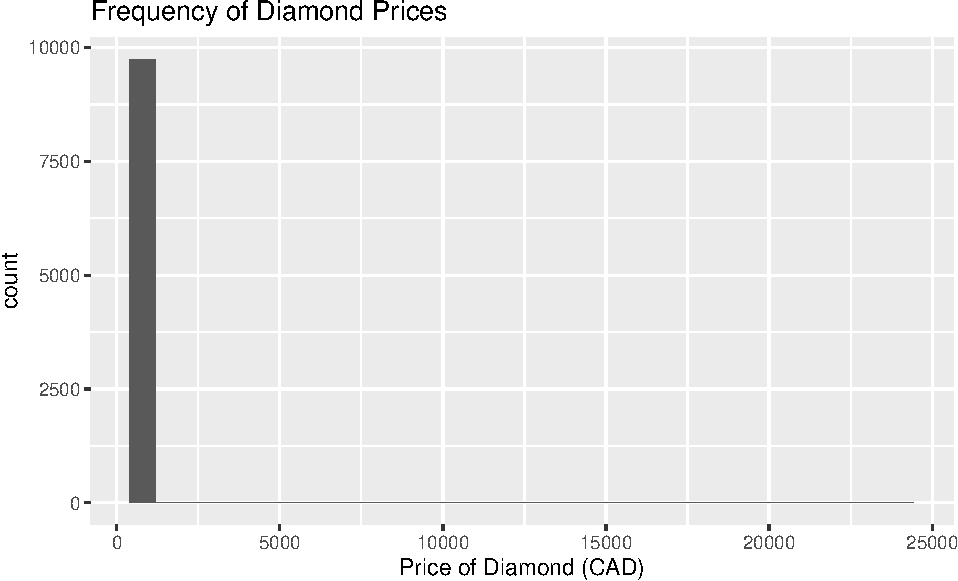
\includegraphics[width=0.8\linewidth]{Methods_and_Results_files/figure-latex/unnamed-chunk-4-1} \end{center}

We can see that the majority of the diamonds have similar price around
1000 CAD with some pricier diamonds scattered on the right. This may be
due to cheaper diamonds being more accessible to both the vendor and
customers. However, this is a limitation of our data, which I will
discuss more in the limitations section.

\begin{center}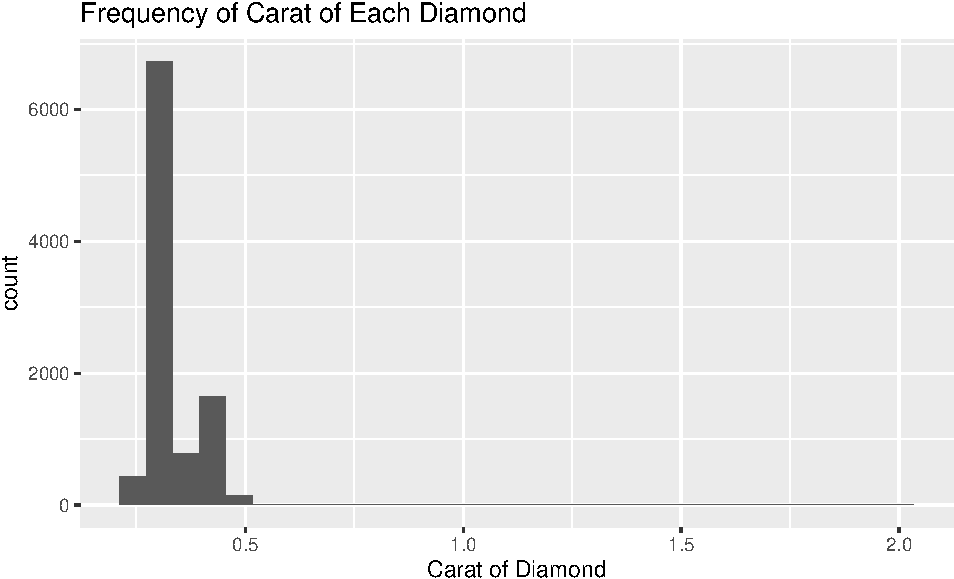
\includegraphics[width=0.8\linewidth]{Methods_and_Results_files/figure-latex/unnamed-chunk-5-1} \end{center}

The distribution of the carat also appears to be skewed to the right,
with a mean of around 0.3. This is also normal as it is more common to
see smaller diamonds as it is a rare resource.

\begin{center}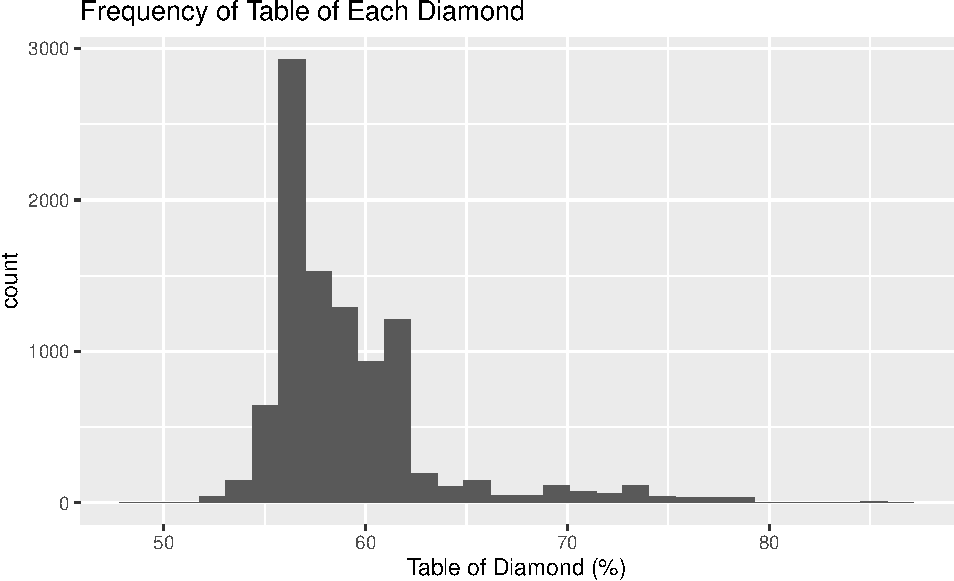
\includegraphics[width=0.8\linewidth]{Methods_and_Results_files/figure-latex/unnamed-chunk-6-1} \end{center}

The table percentage of the diamond appears to be skewed to the right. I
would consider this as normal due to how the diamonds are usually cut to
look appealing. The potential outliers of the table could be caused by
diamonds having different shapes.

\begin{center}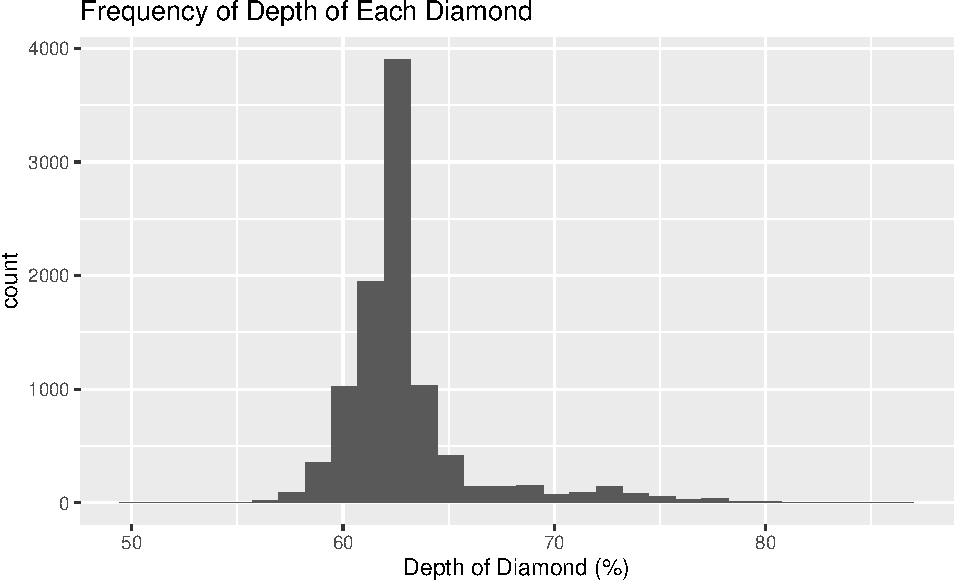
\includegraphics[width=0.8\linewidth]{Methods_and_Results_files/figure-latex/unnamed-chunk-7-1} \end{center}

The depth percentage of the diamond appears to be roughly Normal. I
would consider this as normal due to how the diamonds are usually cut to
look appealing. The potential outliers of the depth could also be caused
by diamonds having different shapes.

Next, I will look into how the prices differ based on each group of our
factors (Shape, cut, color, and clarity)

\begin{center}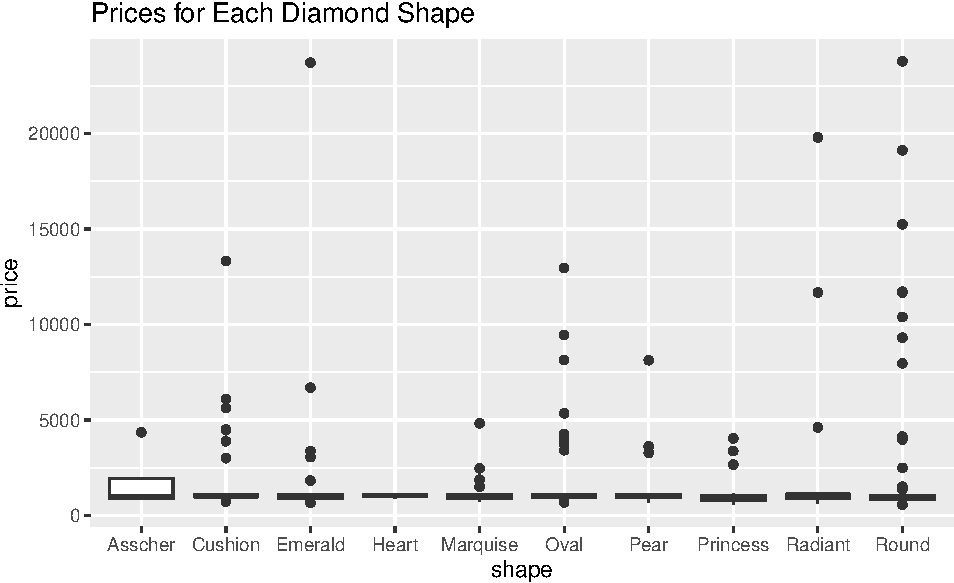
\includegraphics[width=0.8\linewidth]{Methods_and_Results_files/figure-latex/unnamed-chunk-8-1} \end{center}

We can see that for different shapes, the median price is around the
same. The greater price range for round shaped diamond compared to other
shapes may be due its high popularity as shown in Table 2.

\begin{center}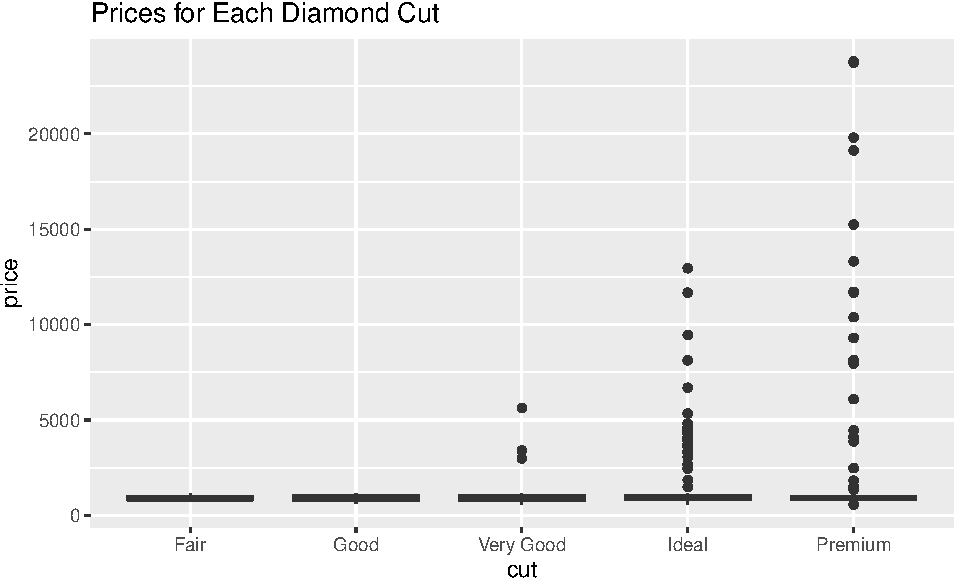
\includegraphics[width=0.8\linewidth]{Methods_and_Results_files/figure-latex/unnamed-chunk-9-1} \end{center}

We can see that even though the different cuts' median prices are
similar, the price range for a premium cut diamond is greater compared
to other cuts. This means that there are more variety in terms of price
when it comes to having an above very good cut.

\begin{center}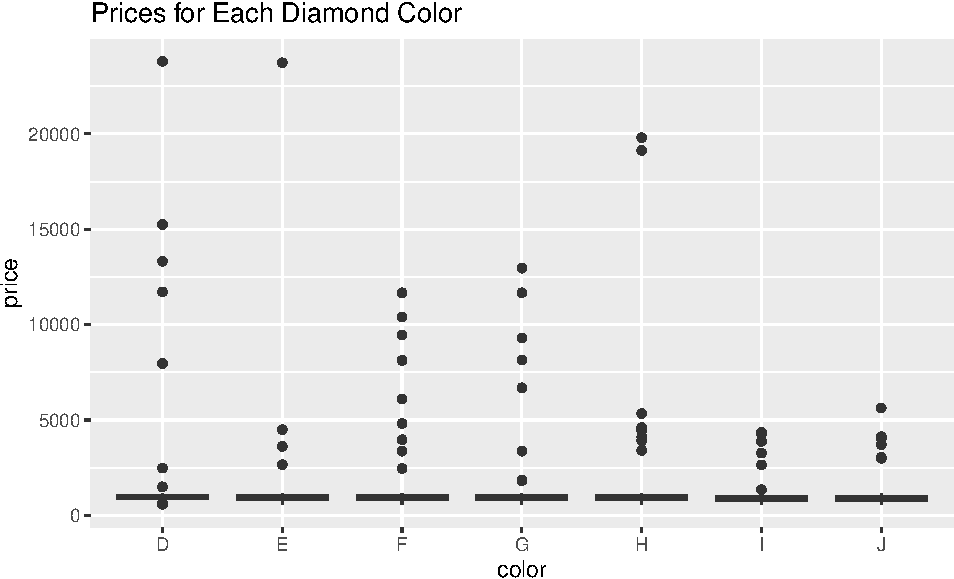
\includegraphics[width=0.8\linewidth]{Methods_and_Results_files/figure-latex/unnamed-chunk-10-1} \end{center}

We can see that for different color, the median price is around the
same. The greater price range for D colored diamond compared to other
shapes may be due it being the best possible color, thus having more
variability.

\begin{center}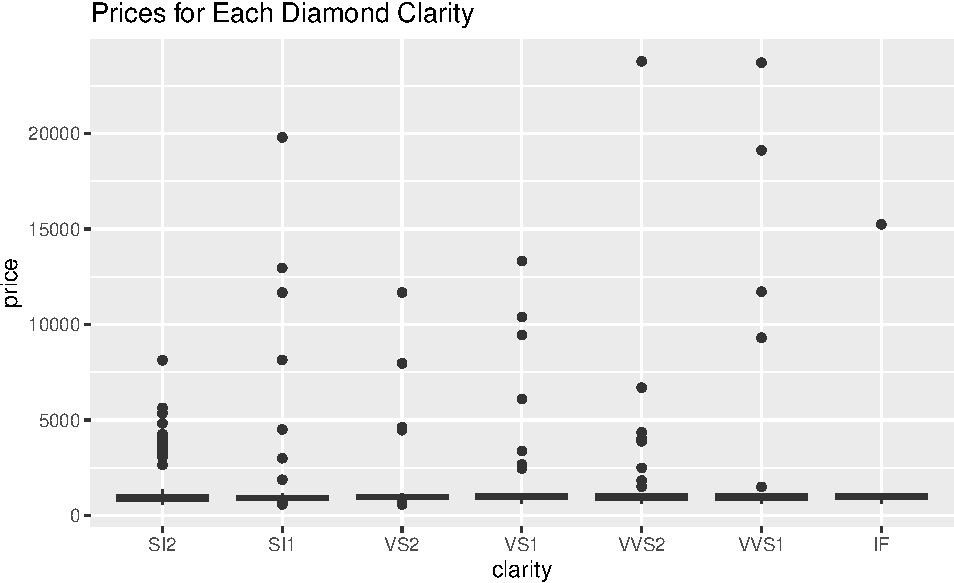
\includegraphics[width=0.8\linewidth]{Methods_and_Results_files/figure-latex/unnamed-chunk-11-1} \end{center}

We can see that for different clarity, the median price is around the
same. We also see that in all clarity levels, there are upper outliers.
This means that despite having different clarity levels, there are still
a variety of diamonds that are expensive.

Next, I will look into how the prices differ based on continuous
variables (table and depth):

\begin{center}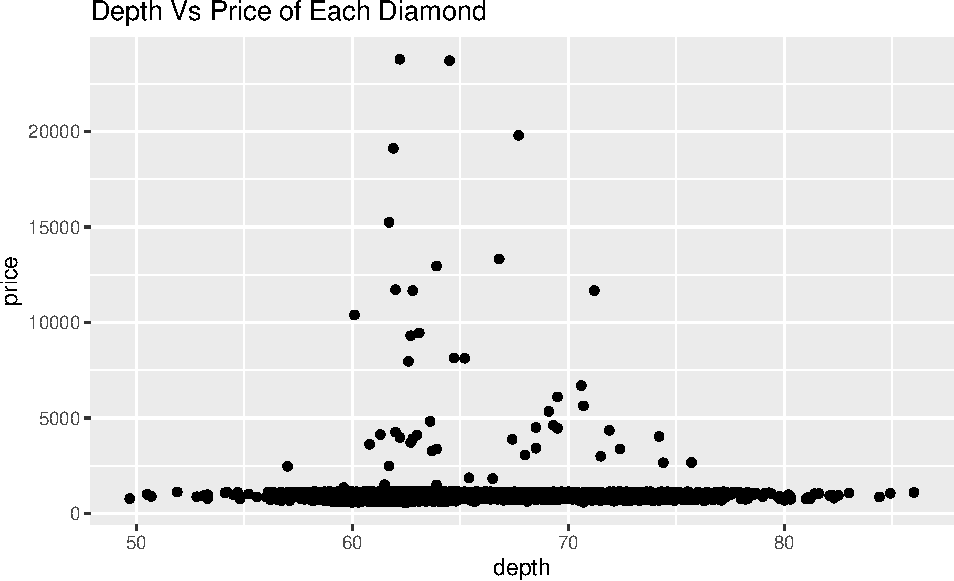
\includegraphics[width=0.8\linewidth]{Methods_and_Results_files/figure-latex/unnamed-chunk-12-1} \end{center}

We see that in general, there is a cheap option for all different
depths. However, around the mean depth (63\%), we see a more more
expensive diamond options

\begin{center}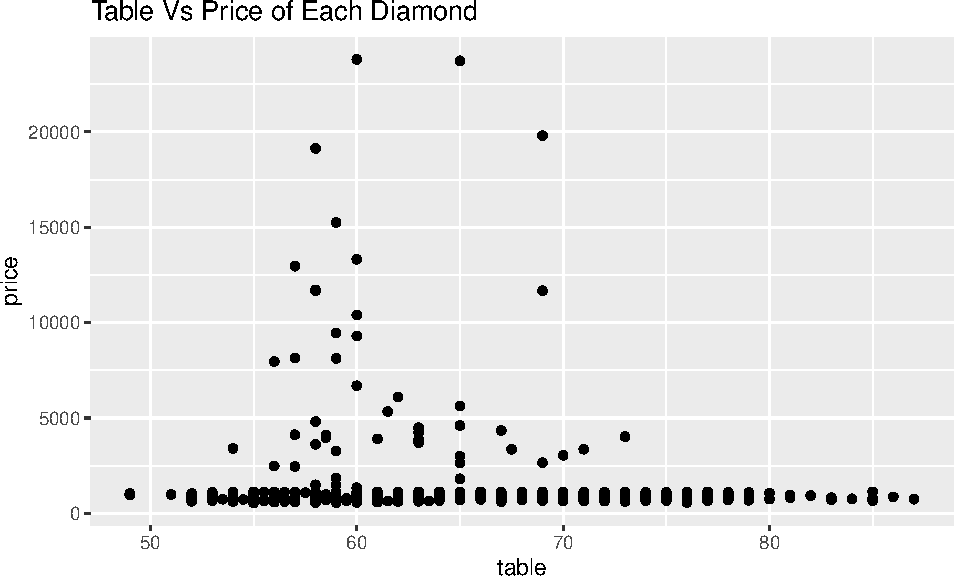
\includegraphics[width=0.8\linewidth]{Methods_and_Results_files/figure-latex/unnamed-chunk-13-1} \end{center}

We see a pretty similar result as the depth vs price table, where all
tables have a cheap option and have a more expensive options around the
mean table (59\%).

Based on the box plot and scatter plots, we see that there are a variety
of diamond prices for each category levels.

\hypertarget{preliminary-results}{%
\subsection{Preliminary Results}\label{preliminary-results}}

To be able to find out what other variables influence the value of a
diamond, I will create scatter plots of carat and price grouped by each
categorical variables (cut, color, clarity, and shape)

\begin{center}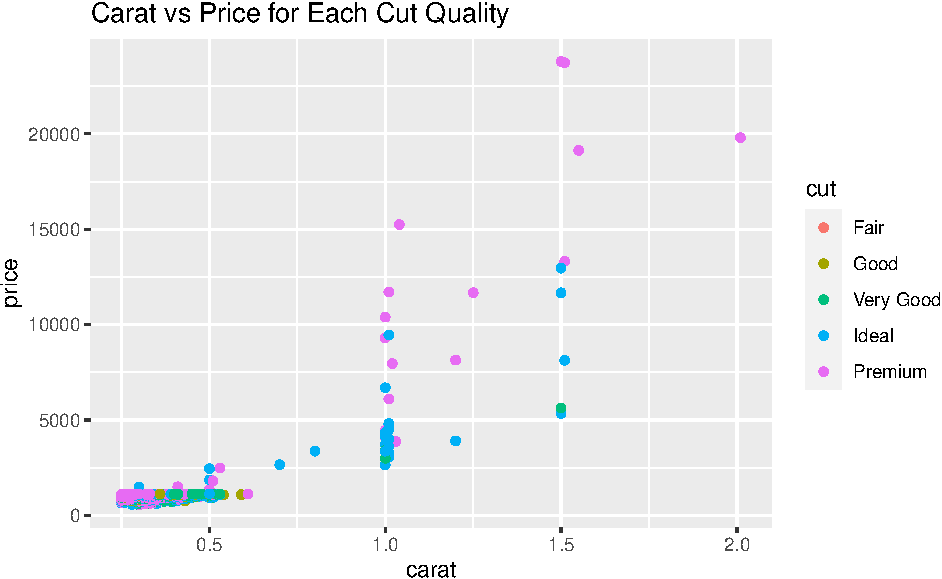
\includegraphics[width=0.8\linewidth]{Methods_and_Results_files/figure-latex/unnamed-chunk-14-1} \end{center}

Besides the bottom left corner, we see that there are more Ideal and
especially Premium cut diamonds having higher price as carat increases.
The Ideal cut diamonds seem to have a linear relationship between carat
and price while the premium cut diamonds seem to have an rough
exponential relationship between carat and price.

\begin{center}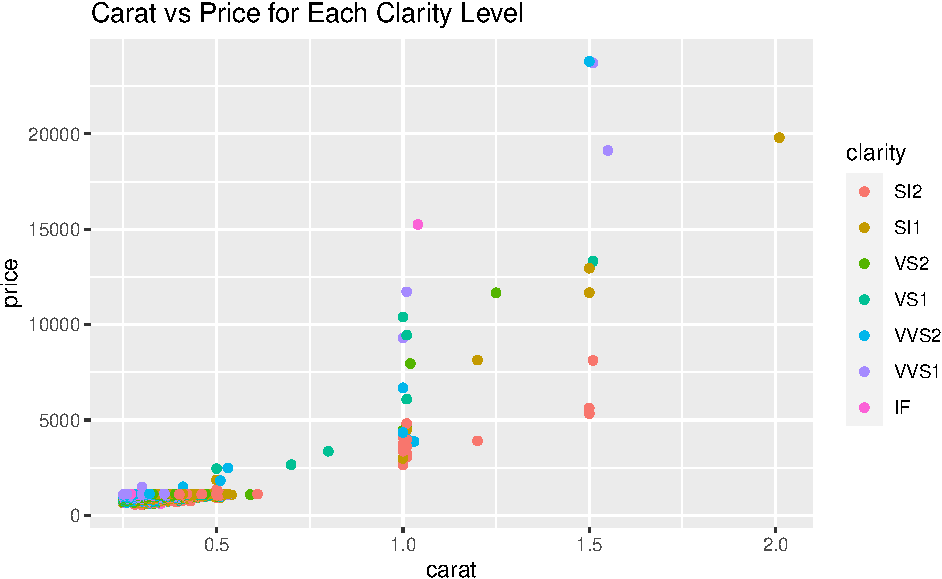
\includegraphics[width=0.8\linewidth]{Methods_and_Results_files/figure-latex/unnamed-chunk-15-1} \end{center}

For each clarity level, we see that there is a rough exponential
relationship between carat and price.

\begin{center}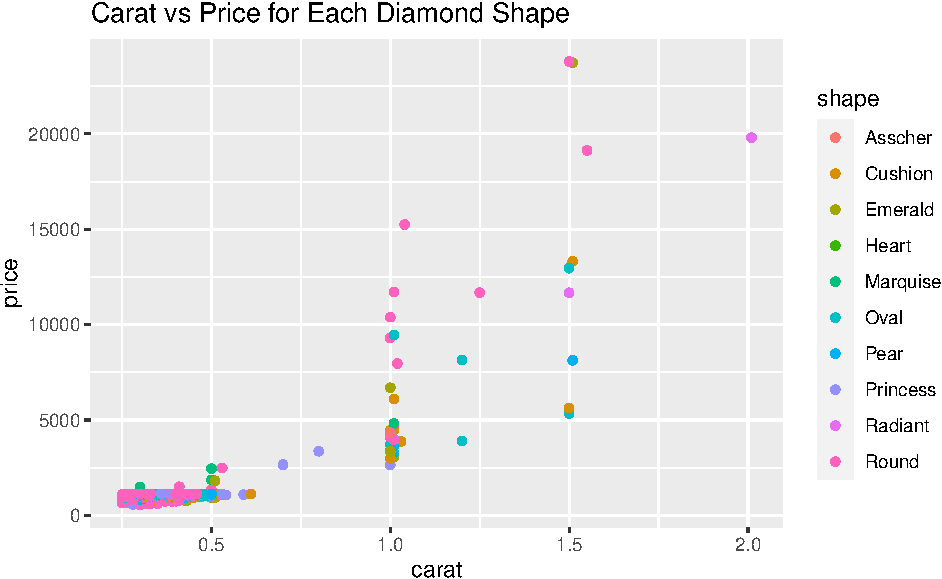
\includegraphics[width=0.8\linewidth]{Methods_and_Results_files/figure-latex/unnamed-chunk-16-1} \end{center}

We see a rough exponential relationship between carat and price for each
diamond shape.

Now, we want to check the frequencies between two categorical variables:

\begin{center}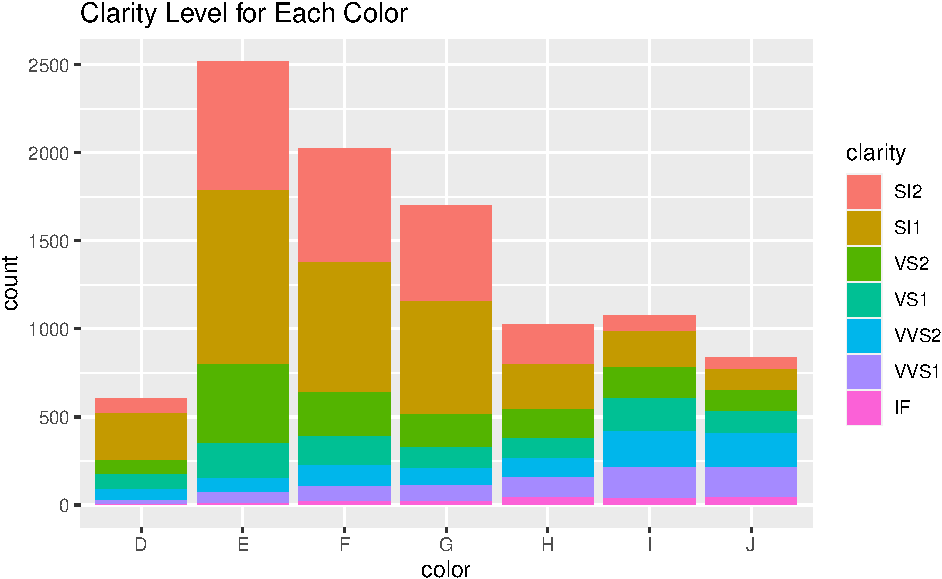
\includegraphics[width=0.8\linewidth]{Methods_and_Results_files/figure-latex/unnamed-chunk-17-1} \end{center}

We see that a combination of decent to average color (E, F) with below
average clarity (SI2, SI1) are preferred more compare to other groups.

\begin{center}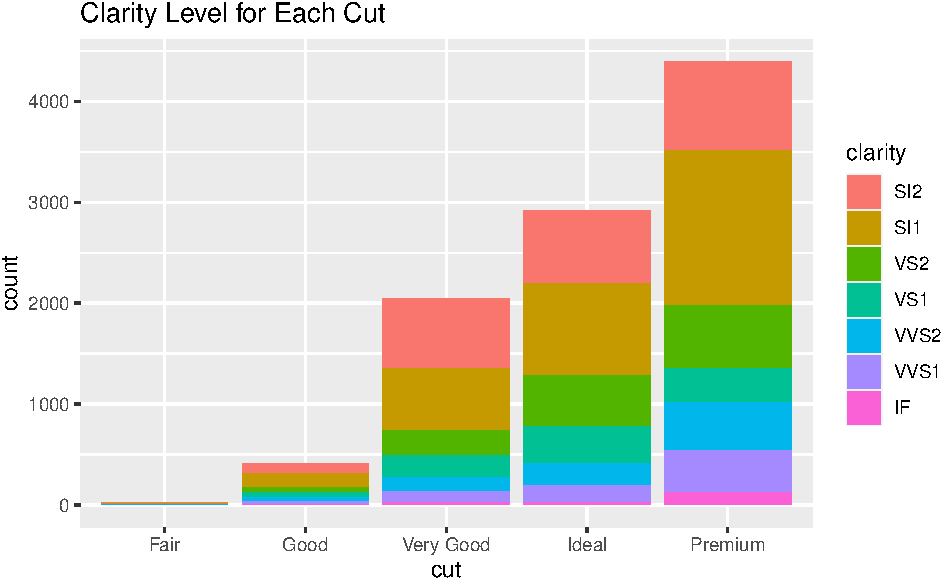
\includegraphics[width=0.8\linewidth]{Methods_and_Results_files/figure-latex/unnamed-chunk-18-1} \end{center}

We see that above very good cut with below average clarity are preferred
more. As the quality of cut increases, there are also more options
across all clarity level.

\begin{center}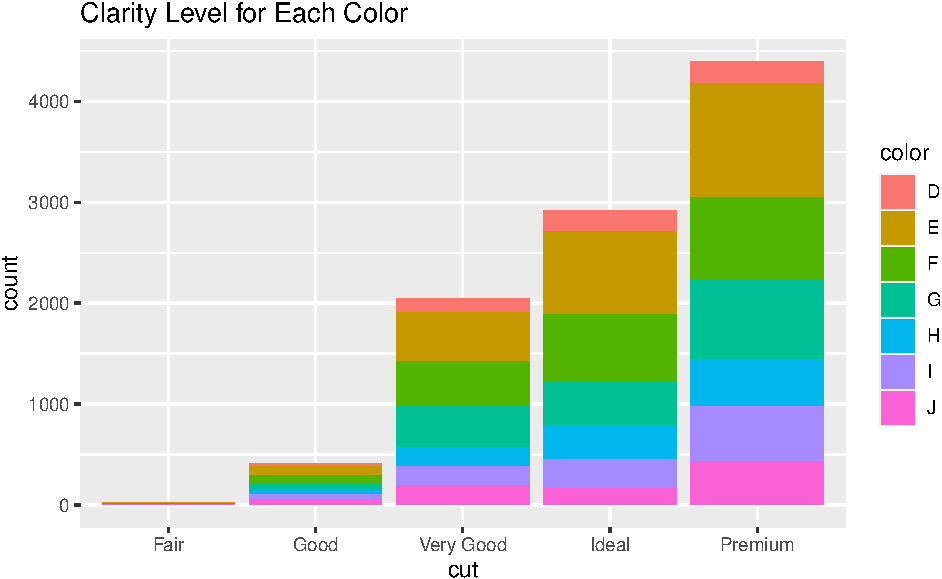
\includegraphics[width=0.8\linewidth]{Methods_and_Results_files/figure-latex/unnamed-chunk-19-1} \end{center}

Similar to the last graph, as the quality of the cut increases, the
count in each color group increases. However, we do see that the most
popular options are above very good cuts with a decent color (E, F).

\hypertarget{conclusions}{%
\subsection{Conclusions}\label{conclusions}}

In this report, my primary guiding question was to investigate what
other qualities, besides from carat, of a diamond influences its value.

Based on the scatter plots, we can say that there seems to exist linear
or exponential relationships for the categorical variables and price,
while more detailed investigation may be needed for continuous variables
such as table and depth.

Based on the stacked bar plots, we can see what pair of categories are
more popular and which category do people care more about (which seems
to be cut, color, and then clarity).

\hypertarget{limitations}{%
\subsection{Limitations}\label{limitations}}

Overall, the most noticeable limitation of this project is that the
diamond prices are not normally distributed. This data majorily consists
of cheaper diamonds within a similar range. This may cause some
variables being underrepresented when they actually influence the value
of a diamond more. This limitation may be caused by how the data was
obtained. As the table was a dynamic table, the parsing process was made
more difficult as it required more manual work in changing the path to
request the data. This may caused us to miss some data that could be
crucial to this project.

\hypertarget{future-steps}{%
\subsection{Future Steps}\label{future-steps}}

Although the data we collected from Brilliant Earth did not fully clear
up our question of which factors influence the value of a diamond, it
still provided interesting and elementary insights.

As aforementioned, the skewness of the price may be a huge problem as I
progress through this project. A possible way to solve this issue is by
introducing different sources, simulating data, or using bootstrapping
methods.

Another area I want to look into is whether popular combinations of
diamond characteristics increase its value. As shown in the bar plots of
the preliminary results, we see that Premium Cut with SI1 clarity seems
to be more popular. Thus, I would want to look into whether a Premium
Cut with SI1 clarity has a higher value compared to a less popular
combination, ex: Very Good cut with SI1 clarity.

\end{document}
